\cleardoublepage
\section{数值测试}
\label{sec:FINALTest}
在用 C++ 代码分别写完算法 \ref{alg:FINALDLSsplineApproximation}、
\ref{alg:FINALppSSF} 和 \ref{alg:FINALBSSF} 所对应的函数后,
我们将其与 Baltamatica 框架结合,使得函数 spap2、csaps 和 spaps
载入 Baltamatica 后,能在 m 文件中被使用。

我们的目的是追求和 Matlab 一样的计算精度和效率,力求做到更好。
故我们采用 Matlab 中的精度结果和效率结果作为精确解,以此来计算
Baltamatica 中计算精度和效率的误差。

矩阵$C_{M}$和$C_{B}$的相对误差定义为
\begin{equation}
  \label{eq:FINALaccerror}
  e_{\texttt{rel}} := \frac{\left\|C_{B} - C_{M}\right\|_{\infty}}{\left\|C_{M}\right\|_{\infty}},
\end{equation}
这里$C_{M}$是Matlab计算得到的结果,$C_{B}$是 Baltamatica 计算得到的结果。
计算效率定义为
\begin{equation}
  \label{eq:FINALtimeerror}
  E := \frac{t_M}{t_B},
\end{equation}
这里$t_{M}$是Matlab的计算耗时,$t_{B}$是 Baltamatica 对相同函数的计算耗时。

下面我们选取两条曲线和其附近的一些数据点,
用spap2、csaps和spaps函数分别对它们进行拟合。
\subsection{拟合$y=\sin x,\ x\in[0,2\pi]$}
\label{sec:FINALsinx}

我们考虑拟合点列$\{(x_{i},y_{i})\}_{i=1}^{N}$,其中
$y_{i}:=\sin x_{i}+\varepsilon_{i}$,
$\varepsilon_{i}$是一个小扰动。

\subsubsection{spap2}
\label{subsubsec:spap2sinx}
本测试中,对不同规格的$N$,取
\begin{align*}
  x_{i}=\frac{2\pi}{N-1} (i-1),
  \quad &i=1,2,\cdots,N,\\
  w_{1}=w_{N}=100,\quad w_{i}=1, \ &i=2,3,\cdots,N-1.
\end{align*}
取$\sigma_{i},\ i=1,2,\cdots,N$为正态分布的随机数,固定它们并令
\begin{align*}
  \varepsilon_{i}=0.01\sigma_{i},\
  y_{i}=\sin x_{i}+\varepsilon_{i},\quad i=1,2,\cdots,N.
\end{align*}
取$k=6$,$n=N/10+5$。取$\mathbf{t}$满足
\begin{equation*}
  t_{1}=t_{2}=\cdots=t_{k}=0,
  \quad
  t_{i+k}=\frac{20\pi}{N} i,\ i=1,2,\cdots,n-k,
  \quad
  t_{n+1}=t_{n+2}=\cdots=t_{n+k}=2\pi.
\end{equation*}

根据算法 \ref{alg:FINALDLSsplineApproximation},输入上述的
$\mathbf{t}, k, \mathbf{x}, \mathbf{y}, \mathbf{w}$,我们得到了样条函数
$f$。我们可以测试执行此算法的精度和效率。精度测试选取了
样条的节点\texttt{knots},B 样条基函数对应的系数\texttt{coefs},以及样条在
特殊点列上的取值\texttt{values}进行误差分析。效率测试将$\sigma_{i}$完全随机,
测试运行 spap2 函数所花的时间。

该测试在一台Linux系统虚拟机上进行,
本地为一台配备第11代英特尔酷睿i7-1165G7处理器
(主频为2.80 GHz)的笔记本电脑。精度测试结果见
表 \ref{tab:FINALspap2sinxacc},效率测试结果见
表 \ref{tab:FINALspap2sinxtime}。

\begin{table}[htbp]
  \centering
  \caption{\label{tab:FINALspap2sinxacc}spap2函数在拟合$y=\sin x$时的精度测试}
  \begin{tabular}{cccc}
    \hline
    $N$& 1e2 & 1e3 & 1e4\\
    \hline
    $e_{\texttt{knots}}$&0& 1.4136e-16& 1.4136e-16\\
    $e_{\texttt{coefs}}$&2.6877e-15& 4.6558e-15&8.9817e-15\\
    $e_{\texttt{values}}$&8.8834e-16&7.8109e-16&1.3365e-15\\
    \hline
  \end{tabular}
\end{table}

\begin{table}[htbp]
  \centering
  \caption{\label{tab:FINALspap2sinxtime}spap2函数在拟合$y=\sin x$时的效率测试}
  \begin{tabular}{ccccc}
    \hline
    $N$&1e2&1e3&1e4&1e5\\
    \hline
    Baltamatica CPU耗时(s)&0.001013&0.010494&0.403234&77.8079\\
    Matlab CPU耗时(s)&0.001146&0.006996&0.202075&89.6976\\
    $E$&113.1\%&66.7\%&50.1\%&115.3\%\\
    \hline
  \end{tabular}
\end{table}

对不同的$N$,绘制生成的样条图像,如图 \ref{fig:FINALspap2sinx} 所示。

\begin{figure}[h]  
  \centering   
  \begin{minipage}{0.3\textwidth}  
    \centering  
    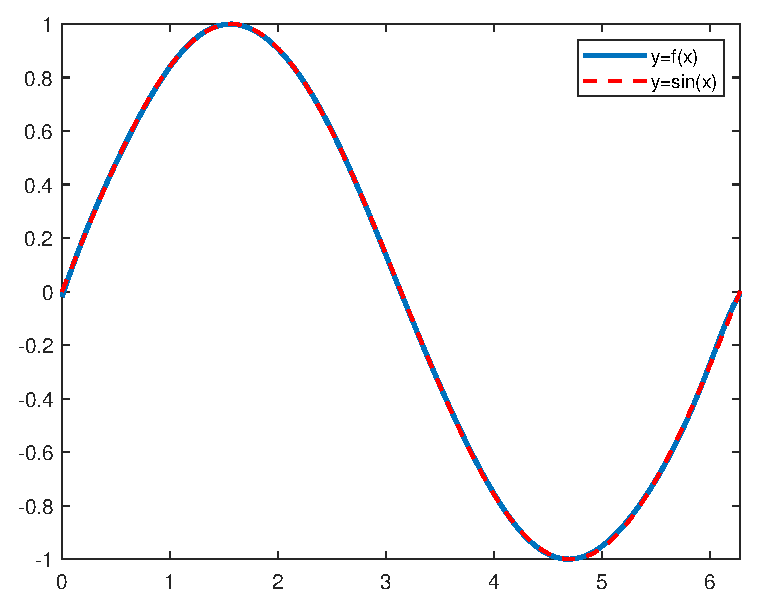
\includegraphics[width=\linewidth]{eps/spap2sinx100.eps}  
    \caption*{$N=100$}  
  \end{minipage}  
  \hfill  
  \begin{minipage}{0.3\textwidth}  
    \centering  
    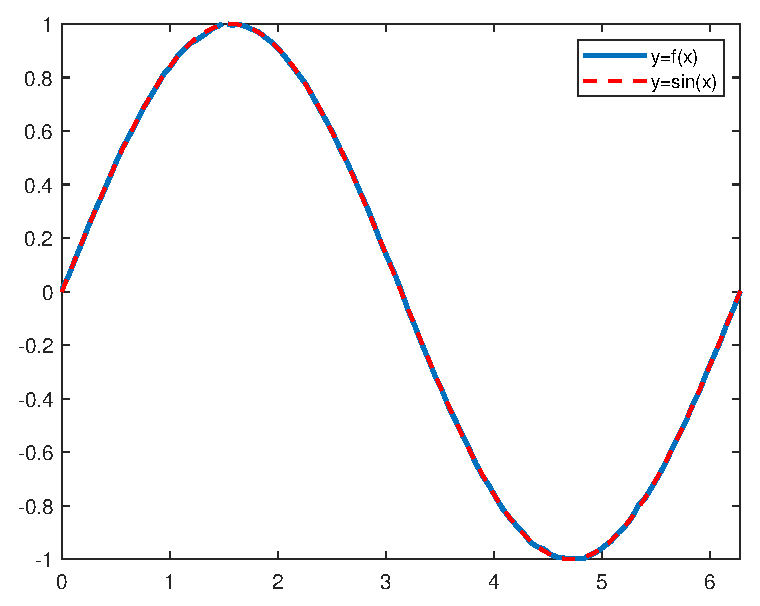
\includegraphics[width=\linewidth]{eps/spap2sinx1000.eps}  
    \caption*{$N=1000$}  
  \end{minipage}
  \hfill  
  \begin{minipage}{0.3\textwidth}  
    \centering  
    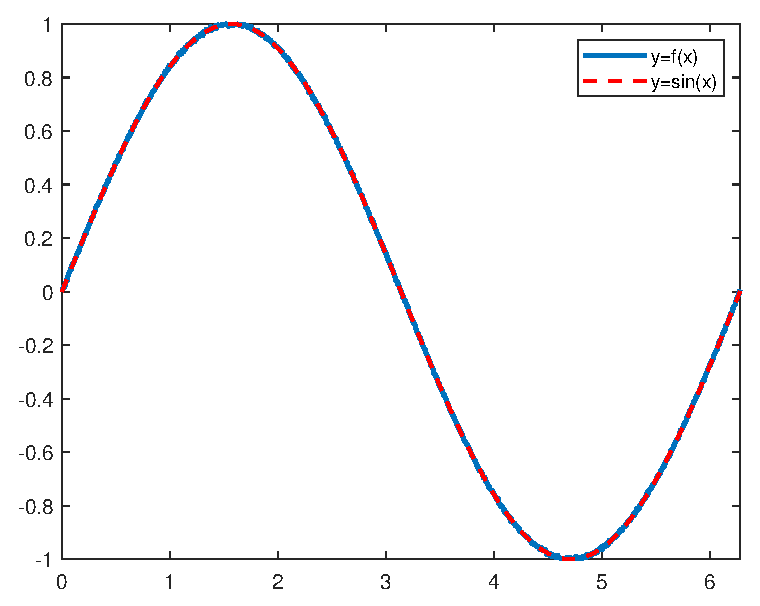
\includegraphics[width=\linewidth]{eps/spap2sinx10000.eps}  
    \caption*{$N=10000$}  
  \end{minipage}   
  \caption{针对不同规模的数据点,Matlab 中通过 spap2 函数
    拟合$y=\sin x$得到的样条}
  \label{fig:FINALspap2sinx}  
\end{figure}

\subsubsection{csaps}
\label{subsubsec:csapssinx}
本测试中,对不同规格的$N$,取
\begin{align*}
  x_{i}=\frac{2\pi}{N-1} (i-1),
  \quad &i=1,2,\cdots,N,\\
  w_{1}=w_{N}=100,\quad w_{i}=1, \ &i=2,3,\cdots,N-1.
\end{align*}
取$\sigma_{i},\ i=1,2,\cdots,N$为$(0,1)$之间均匀分布的随机数,
固定它们并令
\begin{align*}
  \varepsilon_{i}=0.3(\sigma_{i}-0.5),\
  y_{i}=\sin x_{i}+\varepsilon_{i},\quad i=1,2,\cdots,N.
\end{align*}
取$p=0.4$,$\lambda_{i}$满足
\begin{displaymath}
  \lambda_{\frac{N}{2}}=\lambda_{\frac{N}{2}+1}=100,\quad
  \lambda_{i}=1, i\neq \frac{N}{2},\frac{N}{2}+1.
\end{displaymath}

根据算法 \ref{alg:FINALppSSF},输入上述的
$\mathbf{x}, \mathbf{y}, \mathbf{w}, \lambda, p$,我们得到了样条函数
$f$。我们可以测试执行此算法的精度和效率。精度测试选取了
样条的节点\texttt{breaks},分段多项式对应的系数\texttt{coefs},以及样条在
特殊点列上的取值\texttt{values}进行误差分析。效率测试将$\sigma_{i}$完全随机,
测试运行 csaps 函数所花的时间。

该测试在一台Linux系统虚拟机上进行,
本地为一台配备第11代英特尔酷睿i7-1165G7处理器
(主频为2.80 GHz)的笔记本电脑。
精度测试结果见
表 \ref{tab:FINALcsapssinxacc},效率测试结果见
表 \ref{tab:FINALcsapssinxtime}。

\begin{table}[htbp]
  \centering
  \caption{\label{tab:FINALcsapssinxacc}csaps函数在拟合$y=\sin x$时的精度测试}
  \begin{tabular}{cccc}
    \hline
    $N$& 1e2 & 1e3 & 1e4\\
    \hline
    $e_{\texttt{breaks}}$& 1.4136e-16& 1.4136e-16& 1.4136e-16\\
    $e_{\texttt{coefs}}$&5.9487e-13&6.5222e-10&9.3129e-07\\
    $e_{\texttt{values}}$& 1.9127e-13&7.4260e-11&3.1651e-08\\
    \hline
  \end{tabular}
\end{table}

\begin{table}[htbp]
  \centering
  \caption{\label{tab:FINALcsapssinxtime}csaps函数在拟合$y=\sin x$时的效率测试}
  \begin{tabular}{ccccc}
    \hline
    $N$&1e2&1e3&1e4&1e5\\
    \hline
    Baltamatica CPU耗时(s)&0.000192&0.000724&0.007596&0.053593\\
    Matlab CPU耗时(s)&0.000467&0.001121&0.008273&0.071413\\
    $E$&243.2\%&154.8\%&108.9\%&133.3\%\\
    \hline
  \end{tabular}
\end{table}
对不同的$N$,绘制生成的样条图像,如图 \ref{fig:FINALcsapssinx} 所示。

\begin{figure}[h]  
  \centering   
  \begin{minipage}{0.3\textwidth}  
    \centering  
    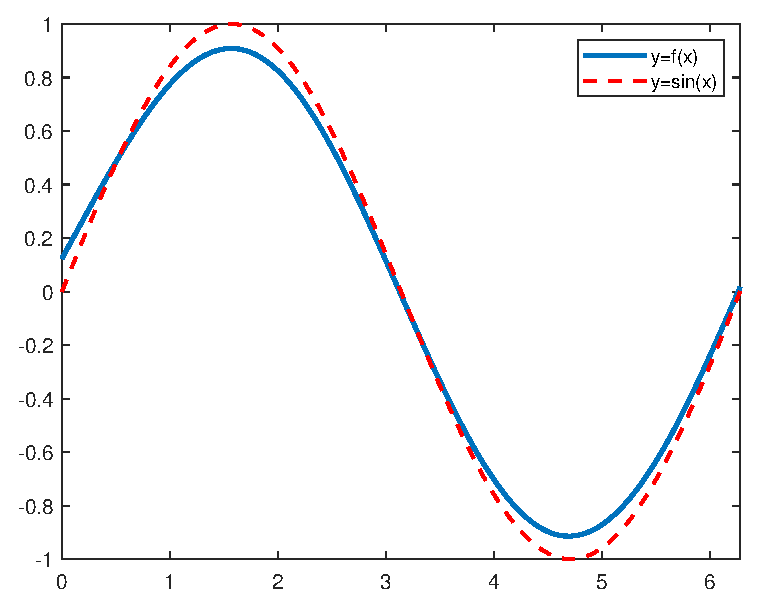
\includegraphics[width=\linewidth]{eps/csapssinx100.eps}  
    \caption*{$N=100$}  
  \end{minipage}  
  \hfill  
  \begin{minipage}{0.3\textwidth}  
    \centering  
    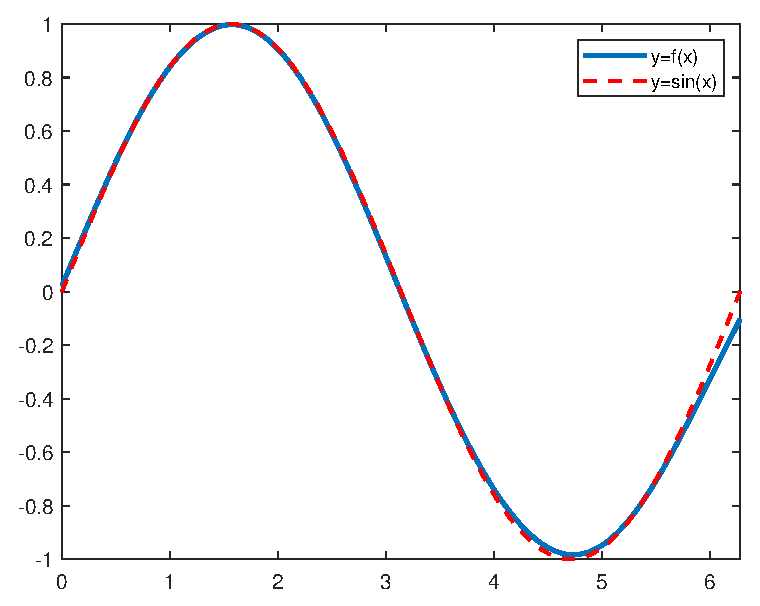
\includegraphics[width=\linewidth]{eps/csapssinx1000.eps}  
    \caption*{$N=1000$}  
  \end{minipage}
  \hfill  
  \begin{minipage}{0.3\textwidth}  
    \centering  
    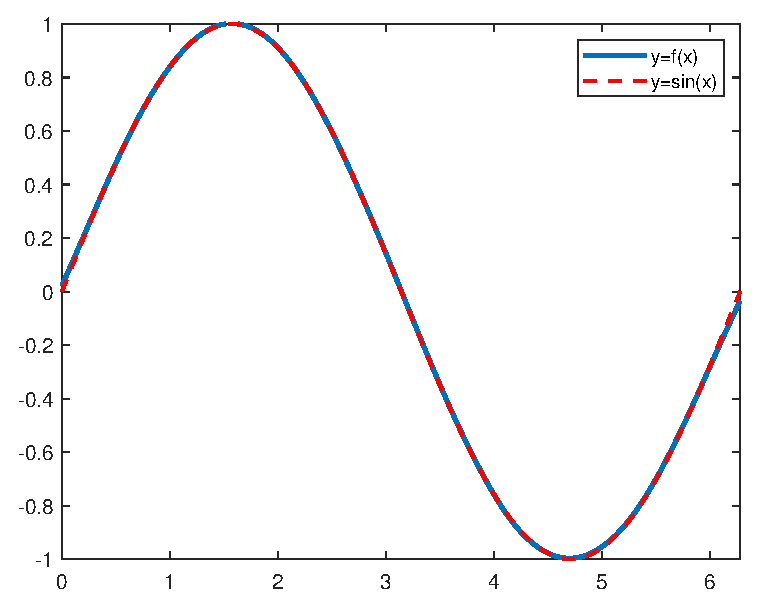
\includegraphics[width=\linewidth]{eps/csapssinx10000.eps}  
    \caption*{$N=10000$}  
  \end{minipage}   
  \caption{针对不同规模的数据点,Matlab 中通过 csaps 函数拟合$y=\sin x$得到的样条}
  \label{fig:FINALcsapssinx}  
\end{figure}

\subsubsection{spaps}
\label{subsubsec:spapssinx}
本测试中,对不同规格的$N$,取
\begin{align*}
  x_{i}=\frac{2\pi}{N-1} (i-1),
  \quad &i=1,2,\cdots,N,\\
  w_{i}=\frac{1}{2\pi},\quad &i=1,2,\cdots,N.
\end{align*}
取$\sigma_{i},\ i=1,2,\cdots,N$为$(0,1)$之间均匀分布的随机数,
固定它们并令
\begin{align*}
  \varepsilon_{i}=0.02(\sigma_{i}-0.5),\
  y_{i}=\sin x_{i}+\varepsilon_{i},\quad i=1,2,\cdots,N.
\end{align*}
取$m=2,\ S=0.05^{2}\times2\pi$,$\lambda_{i}$满足
\begin{displaymath}
  \lambda_{\frac{N}{2}}=100,\quad
  \lambda_{i}=1, i\neq \frac{N}{2}.
\end{displaymath}

根据算法 \ref{alg:FINALBSSF},输入上述的
$\mathbf{x}, \mathbf{y}, \mathbf{w}, \lambda, m,S$,我们得到了样条函数
$f$和平滑参数$\rho$。我们可以测试执行此算法的精度和效率。
精度测试选取了
样条的节点\texttt{knots},B 样条基函数对应的系数\texttt{coefs},
样条在某些点处的取值\texttt{values},以及平滑参数\texttt{rho}进行误差分析。
效率测试将$\sigma_{i}$完全随机,
测试运行 spaps 函数所花的时间。

该测试在一台配备AMD R9-7945HX处理器(主频为2.50 GHz)的笔记本电脑上进行。
精度测试结果见
表 \ref{tab:FINALspapssinxacc},效率测试结果见
表 \ref{tab:FINALspapssinxtime}。

注意到表 \ref{tab:FINALspapssinxacc} 中当$N=$1e4时,$e_{\texttt{rho}}$
的精度损失严重,其原因可能是\texttt{rho}的精确值本身很大
(Matlab 上结果为1.822725407145163e+11)。

\begin{table}[htbp]
  \centering
  \caption{\label{tab:FINALspapssinxacc}spaps函数在拟合$y=\sin x$时的精度测试}
  \begin{tabular}{cccc}
    \hline
    $N$& 1e2 & 1e3 & 1e4\\
    \hline
    $e_{\texttt{knots}}$&1.4136e-16&1.4136e-16&1.4136e-16\\
    $e_{\texttt{coefs}}$&9.1338e-13& 2.8246e-09&9.7282e-09\\
    $e_{\texttt{values}}$&4.3030e-14&4.2871e-11&5.0138e-09\\
    $e_{\texttt{rho}}$&9.8470e-13&9.0219e-10& 1.9097e-06\\
    \hline
  \end{tabular}
\end{table}

\begin{table}[htbp]
  \centering
  \caption{\label{tab:FINALspapssinxtime}spaps函数在拟合$y=\sin x$时的效率测试}
  \begin{tabular}{ccccc}
    \hline
    $N$&1e2&1e3&1e4&1e5\\
    \hline
    Baltamatica CPU耗时(s)&0.000132&0.000738&0.004938&0.052357\\
    Matlab CPU耗时(s)&0.001151&0.001499&0.010299&0.113626\\
    $E$&872.0\%&203.1\%&208.6\%&217.0\%\\
    \hline
  \end{tabular}
\end{table}

对不同的$N$,绘制生成的样条图像,如图 \ref{fig:FINALspapssinx} 所示。

\begin{figure}[h]  
  \centering   
  \begin{minipage}{0.3\textwidth}  
    \centering  
    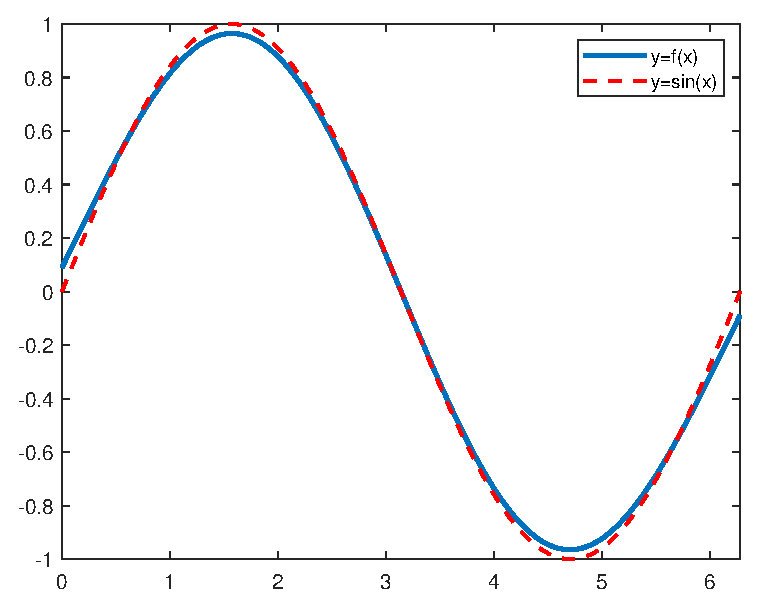
\includegraphics[width=\linewidth]{eps/spapssinx100.eps}  
    \caption*{$N=100$}  
  \end{minipage}  
  \hfill  
  \begin{minipage}{0.3\textwidth}  
    \centering  
    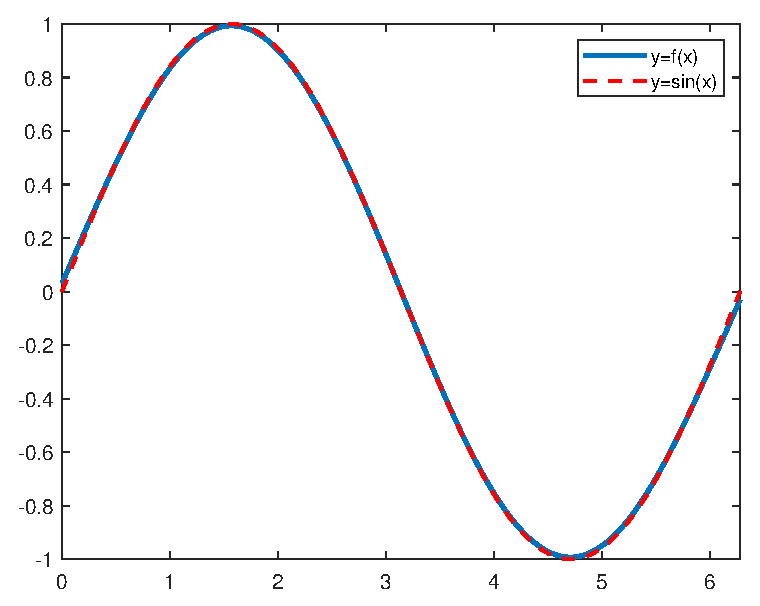
\includegraphics[width=\linewidth]{eps/spapssinx1000.eps}  
    \caption*{$N=1000$}  
  \end{minipage}
  \hfill  
  \begin{minipage}{0.3\textwidth}  
    \centering  
    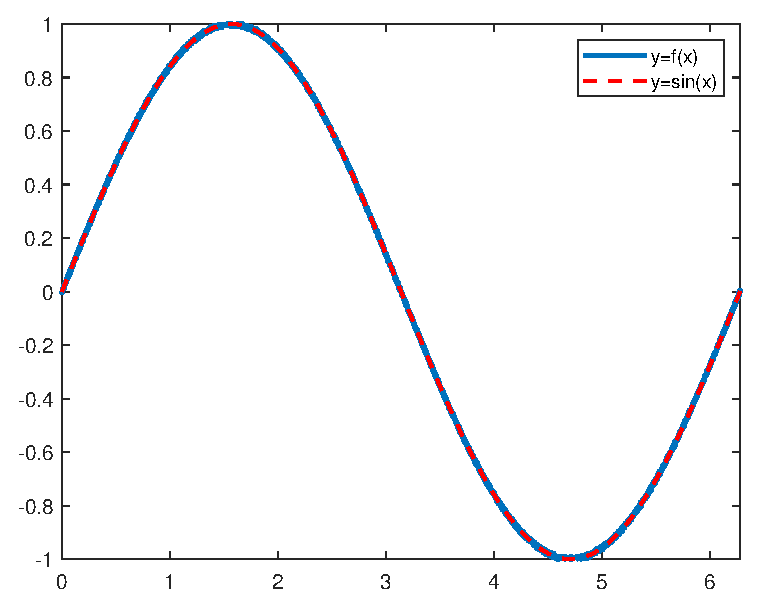
\includegraphics[width=\linewidth]{eps/spapssinx10000.eps}  
    \caption*{$N=10000$}  
  \end{minipage}   
  \caption{针对不同规模的数据点,Matlab 中通过 spaps 函数拟合$y=\sin x$得到的样条}
  \label{fig:FINALspapssinx}  
\end{figure}


\subsection{拟合$y=1/(1+25x^{2}),\ x\in[-1,1]$}
\label{sec:FINALRunge}

类似 \ref{sec:FINALsinx} 节,
考虑拟合点列$\{(x_{i},y_{i})\}_{i=1}^{N}$,其中
$y_{i}:=1/(1+25x_{i}^{2})+\varepsilon_{i}$。

\subsubsection{spap2}
\label{subsubsec:spap2Runge}
取
\begin{align*}
  x_{i}=\frac{2}{N-1} (i-1)-1,\
  w_{i}=1, \quad i=1,2,\cdots,N.
\end{align*}
取$\sigma_{i},\ i=1,2,\cdots,N$为正态分布的随机数,固定它们并令
\begin{align*}
  \varepsilon_{i}=0.001\sigma_{i},\
  y_{i}=\frac{1}{1+25x_{i}^{2}}+\varepsilon_{i},\quad i=1,2,\cdots,N.
\end{align*}
取$k=4$,$n=N/10+3$。取$\mathbf{t}$满足
\begin{equation*}
  t_{1}=t_{2}=\cdots=t_{k}=-1,
  \quad
  t_{i+k}=\frac{20}{N} i-1,\ i=1,2,\cdots,n-k,
  \quad
  t_{n+1}=t_{n+2}=\cdots=t_{n+k}=1.
\end{equation*}

该测试在一台Linux系统虚拟机上进行,
本地为一台配备第11代英特尔酷睿i7-1165G7处理器
(主频为2.80 GHz)的笔记本电脑。精度测试结果见
表 \ref{tab:FINALspap2Rungeacc},效率测试结果见
表 \ref{tab:FINALspap2Rungetime}。

\begin{table}[htbp]
  \centering
  \caption{\label{tab:FINALspap2Rungeacc}spap2函数在拟合$y=\frac{1}{1+25x^{2}}$时的精度测试}
  \begin{tabular}{cccc}
    \hline
    $N$& 1e2 & 1e3 & 1e4\\
    \hline
    $e_{\texttt{knots}}$&1.6653e-16& 1.1102e-16& 1.3878e-16\\
    $e_{\texttt{coefs}}$&3.8773e-16& 1.5478e-15&2.7752e-15\\
    $e_{\texttt{values}}$&1.1266e-16&2.2192e-16& 8.8815e-16\\
    \hline
  \end{tabular}
\end{table}

\begin{table}[htbp]
  \centering
  \caption{\label{tab:FINALspap2Rungetime}spap2函数在拟合$y=\frac{1}{1+25x^{2}}$时的效率测试}
  \begin{tabular}{ccccc}
    \hline
    $N$&1e2&1e3&1e4&1e5\\
    \hline
    Baltamatica CPU耗时(s)&0.000378&0.004915&0.410405&48.3044\\
    Matlab CPU耗时(s)&0.002196&0.006868&0.429961&77.5800\\
    $E$&581.0\%&139.7\%&104.8\%&160.6\%\\
    \hline
  \end{tabular}
\end{table}

对不同的$N$,绘制生成的样条图像,如图 \ref{fig:FINALspap2Runge} 所示。

\begin{figure}[h]  
  \centering   
  \begin{minipage}{0.3\textwidth}  
    \centering  
    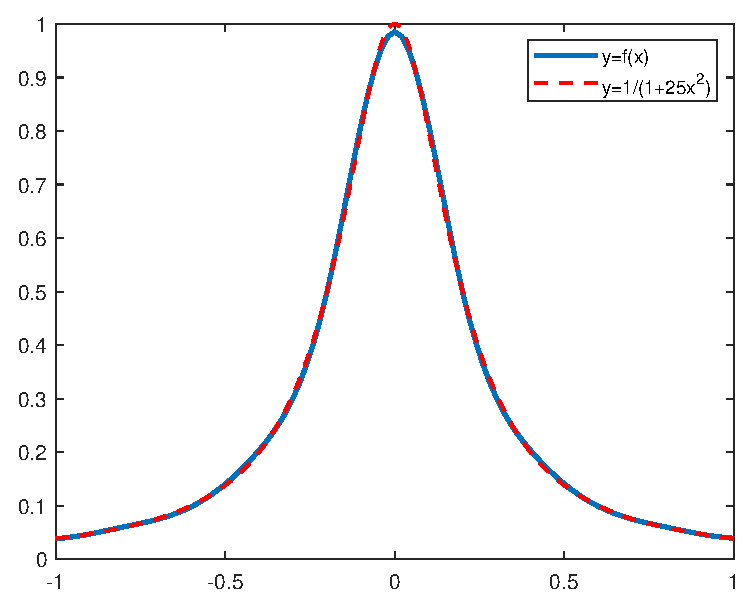
\includegraphics[width=\linewidth]{eps/spap2Runge100.eps}  
    \caption*{$N=100$}  
  \end{minipage}  
  \hfill  
  \begin{minipage}{0.3\textwidth}  
    \centering  
    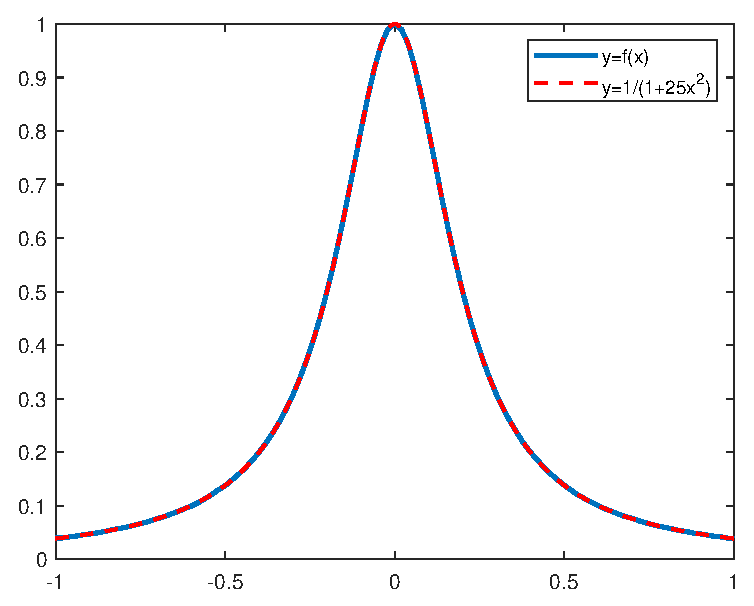
\includegraphics[width=\linewidth]{eps/spap2Runge1000.eps}  
    \caption*{$N=1000$}  
  \end{minipage}
  \hfill  
  \begin{minipage}{0.3\textwidth}  
    \centering  
    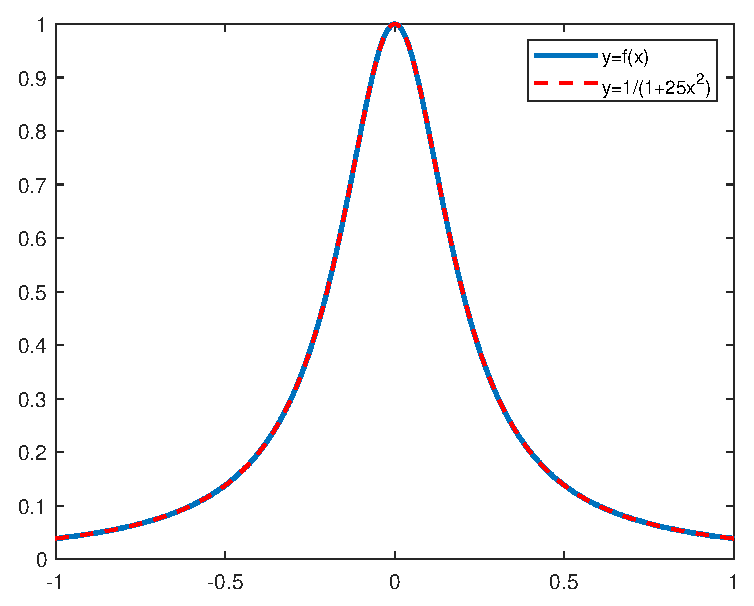
\includegraphics[width=\linewidth]{eps/spap2Runge10000.eps}  
    \caption*{$N=10000$}  
  \end{minipage}   
  \caption{针对不同规模的数据点,Matlab 中通过 spap2 函数拟合$y=\frac{1}{1+25x^{2}}$得到的样条}
  \label{fig:FINALspap2Runge}  
\end{figure}

\subsubsection{csaps}
\label{subsubsec:csapsRunge}
取
\begin{align*}
    x_{i}=\frac{2}{N-1} (i-1)-1,
  w_{i}=1, \quad i=1,2,\cdots,N.
\end{align*}
取$\sigma_{i},\ i=1,2,\cdots,N$为$(0,1)$之间均匀分布的随机数,
固定它们并令
\begin{align*}
  \varepsilon_{i}=0.3(\sigma_{i}-0.5),\
  y_{i}=1/(1+25x^{2})+\varepsilon_{i},\quad i=1,2,\cdots,N.
\end{align*}
取$p=0.4$,$\lambda\equiv 1$。

该测试在一台Linux系统虚拟机上进行,
本地为一台配备第11代英特尔酷睿i7-1165G7处理器
(主频为2.80 GHz)的笔记本电脑。
精度测试结果见
表 \ref{tab:FINALcsapsRungeacc},效率测试结果见
表 \ref{tab:FINALcsapsRungetime}。

\begin{table}[htbp]
  \centering
  \caption{\label{tab:FINALcsapsRungeacc}csaps函数在拟合$y=\frac{1}{1+25x^{2}}$时的精度测试}
  \begin{tabular}{cccc}
    \hline
    $N$& 1e2 & 1e3 & 1e4\\
    \hline
    $e_{\texttt{breaks}}$& 2.2204e-16&  1.2490e-16& 1.6653e-16\\
    $e_{\texttt{coefs}}$&2.0947e-11&1.7485e-08&3.0886e-05\\
    $e_{\texttt{values}}$& 8.4589e-12&4.7706e-09&8.1718e-06\\
    \hline
  \end{tabular}
\end{table}

\begin{table}[htbp]
  \centering
  \caption{\label{tab:FINALcsapsRungetime}csaps函数在拟合$y=\frac{1}{1+25x^{2}}$时的效率测试}
  \begin{tabular}{ccccc}
    \hline
    $N$&1e2&1e3&1e4&1e5\\
    \hline
    Baltamatica CPU耗时(s)&0.000233&0.000776& 0.014466 &0.158469\\
    Matlab CPU耗时(s)&0.001396&0.002666&0.009074&0.130906\\
    $E$&599.1\%&343.6\%&62.7\%&82.6\%\\
    \hline
  \end{tabular}
\end{table}
对不同的$N$,绘制生成的样条图像,如图 \ref{fig:FINALcsapsRunge} 所示。

\begin{figure}[h]  
  \centering   
  \begin{minipage}{0.3\textwidth}  
    \centering  
    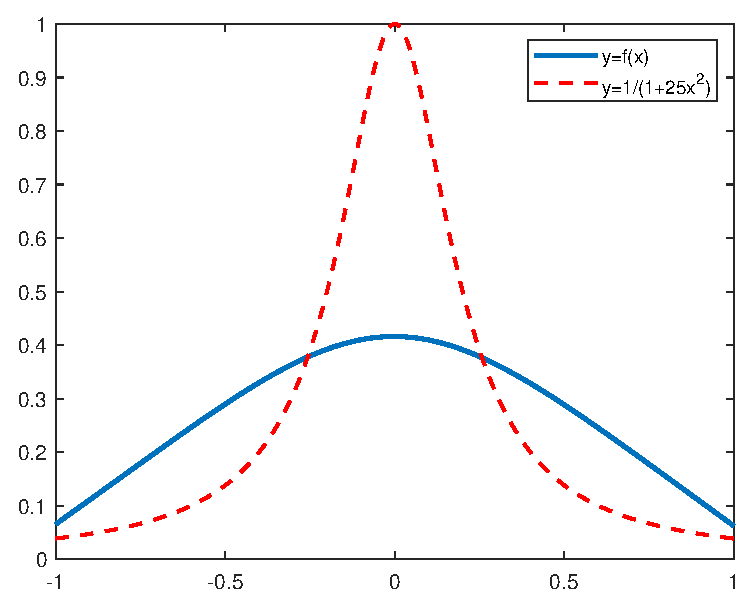
\includegraphics[width=\linewidth]{eps/csapsRunge100.eps}  
    \caption*{$N=100$}  
  \end{minipage}  
  \hfill  
  \begin{minipage}{0.3\textwidth}  
    \centering  
    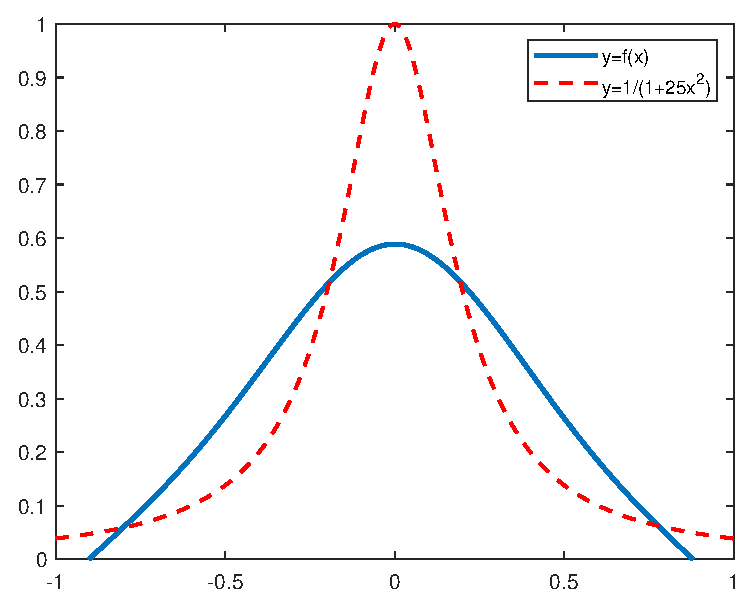
\includegraphics[width=\linewidth]{eps/csapsRunge1000.eps}  
    \caption*{$N=1000$}  
  \end{minipage}
  \hfill  
  \begin{minipage}{0.3\textwidth}  
    \centering  
    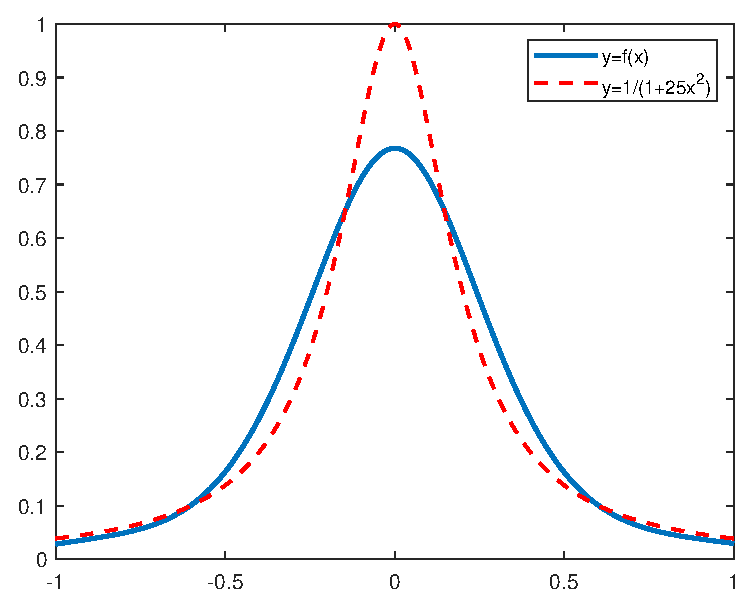
\includegraphics[width=\linewidth]{eps/csapsRunge10000.eps}  
    \caption*{$N=10000$}  
  \end{minipage}   
  \caption{针对不同规模的数据点,Matlab 中通过 csaps 函数拟合$y=\frac{1}{1+25x^{2}}$得到的样条}
  \label{fig:FINALcsapsRunge}  
\end{figure}

\subsubsection{spaps}
\label{subsubsec:spapsRunge}
取
\begin{align*}
  x_{i}=\frac{2}{N-1} (i-1)-1,
 \quad i=1,2,\cdots,N.
\end{align*}
取$\mathbf{w}$使得求和式$E(f)$为积分$\int_{x_{1}}^{x_{N}}|y-f|^{2}$的复化梯形估计。
取$\sigma_{i},\ i=1,2,\cdots,N$为$(0,1)$之间均匀分布的随机数,
固定它们并令
\begin{align*}
  \varepsilon_{i}=0.02(\sigma_{i}-0.5),\
  y_{i}=\sin x_{i}+\varepsilon_{i},\quad i=1,2,\cdots,N.
\end{align*}
取$m=2,\ S=0.05^{2}\times2$,$\lambda_{i}\equiv1$。

该测试在一台配备AMD R9-7945HX处理器(主频为2.50 GHz)的笔记本电脑上进行。
精度测试结果见
表 \ref{tab:FINALspapsRungeacc},效率测试结果见
表 \ref{tab:FINALspapsRungetime}。

在效率测试时,发现 Matlab 在$N=$1e5时稳定报错
“请求的 99998x99998 (149.0GB)数组超过预设的最大数组大小(15.7GB)。”
我们无法测试此时的效率误差;同时,Matlab 在$N=$1e6时有可能报出类似错误,我们
选取了一个正常的运行结果进行效率测试。

\begin{table}[htbp]
  \centering
  \caption{\label{tab:FINALspapsRungeacc}spaps函数在拟合$y=\frac{1}{1+25x^{2}}$时的精度测试}
  \begin{tabular}{cccc}
    \hline
    $N$& 1e2 & 1e3 & 1e4\\
    \hline
    $e_{\texttt{knots}}$&2.2204e-16&1.2490e-16&1.6653e-16\\
    $e_{\texttt{coefs}}$&7.9397e-14& 3.6892e-09&1.3776e-05\\
    $e_{\texttt{values}}$&4.4545e-14& 1.2452e-10& 1.1904e-06\\
    $e_{\texttt{rho}}$&1.3052e-14&2.5906e-10&  1.8551e-05\\
    \hline
  \end{tabular}
\end{table}

\begin{table}[htbp]
  \centering
  \caption{\label{tab:FINALspapsRungetime}spaps函数在拟合$y=\frac{1}{1+25x^{2}}$时的效率测试}
  \begin{tabular}{cccccc}
    \hline
    $N$&1e2&1e3&1e4&1e5&1e6\\
    \hline
    Baltamatica CPU耗时(s)& 0.000160& 0.000898& 0.008436&0.029077&0.780615\\
    Matlab CPU耗时(s)&0.001325&0.002791&0.016567&&1.819144\\
    $E$&828.1\%&310.8\%&196.4\%&&233.0\%\\
    \hline
  \end{tabular}
\end{table}

对不同的$N$,绘制生成的样条图像,如图 \ref{fig:FINALspapsRunge} 所示。

\begin{figure}[h]  
  \centering   
  \begin{minipage}{0.3\textwidth}  
    \centering  
    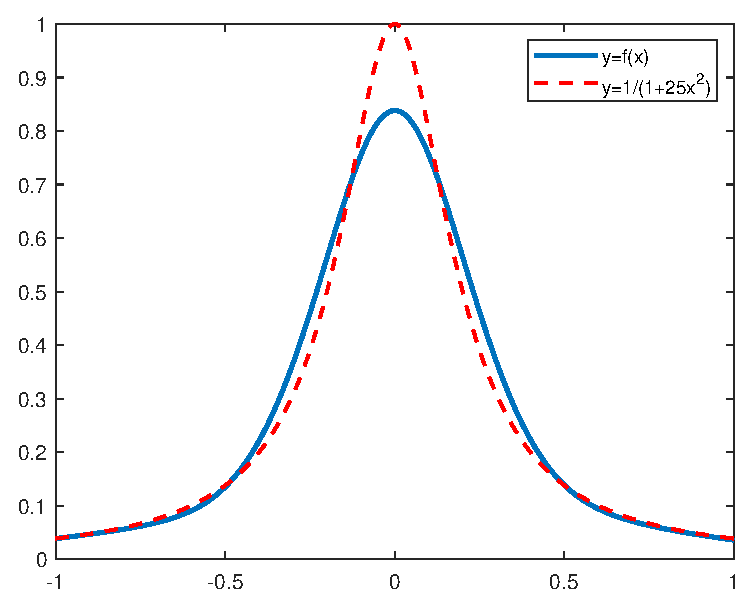
\includegraphics[width=\linewidth]{eps/spapsRunge100.eps}  
    \caption*{$N=100$}  
  \end{minipage}  
  \hfill  
  \begin{minipage}{0.3\textwidth}  
    \centering  
    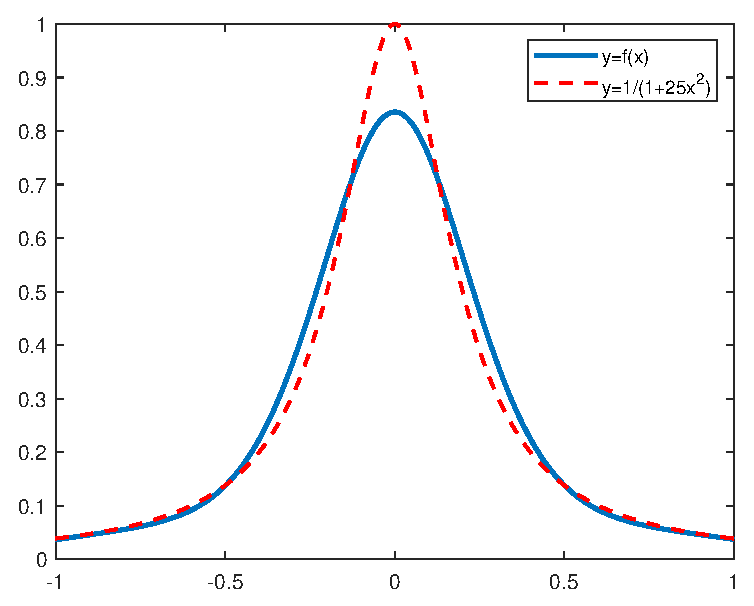
\includegraphics[width=\linewidth]{eps/spapsRunge1000.eps}  
    \caption*{$N=1000$}  
  \end{minipage}
  \hfill  
  \begin{minipage}{0.3\textwidth}  
    \centering  
    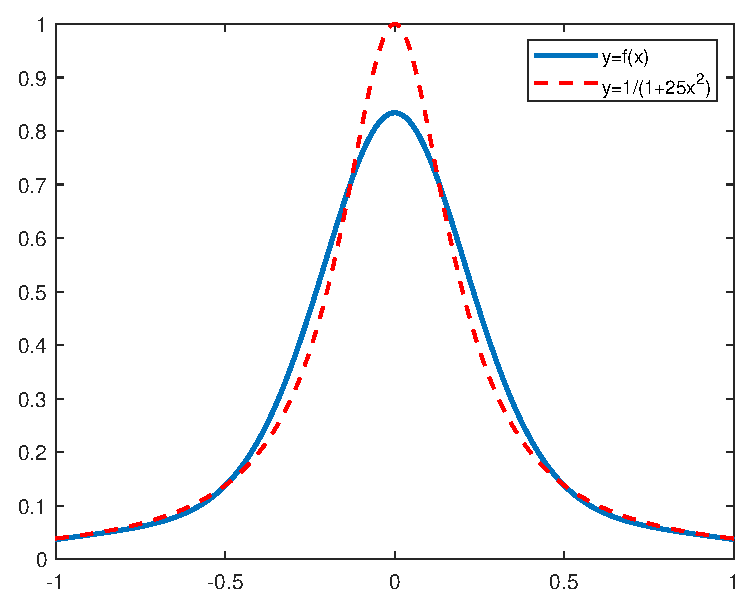
\includegraphics[width=\linewidth]{eps/spapsRunge10000.eps}  
    \caption*{$N=10000$}  
  \end{minipage}   
  \caption{针对不同规模的数据点,Matlab 中通过 spaps 函数拟合$y=\frac{1}{1+25x^{2}}$得到的样条}
  \label{fig:FINALspapsRunge}  
\end{figure}

% \subsection{节标题}

% \subsubsection{小节标题}

% \par 我们可以用includegraphics来插入现有的jpg等格式的图片,如\autoref{fig:zju-logo}。

% \begin{figure}[ht]
%     \centering
%     \includegraphics[width=.4\linewidth]{logo/zju}
%     \caption{\label{fig:zju-logo}浙江大学LOGO}
% \end{figure}

% \par 如\autoref{tab:sample}所示,这是一张自动调节列宽的表格。

% \begin{table}[ht]
%     \caption{\label{tab:sample}自动调节列宽的表格}
%     \begin{tabularx}{\linewidth}{|c|X<{\centering}|}
%         \hline
%         第一列 & 第二列 \\ \hline
%         xxx & xxx \\ \hline
%         xxx & xxx \\ \hline
%         xxx & xxx \\ \hline
%     \end{tabularx}
% \end{table}

% \par 如\autoref{equ:sample},这是一个公式

% \begin{equation}
%     \label{equ:sample}
%     A=\overbrace{(a+b+c)+\underbrace{i(d+e+f)}_{\text{虚数}}}^{\text{复数}}
% \end{equation}

% \par 如\autoref{code:sample}所示,这是一段代码。
% 计算机学院的代码样式可能与其他专业不同,
% 如有需要,可以从计算机学院专业模板中复制相关的代码样式设定。

% \begin{lstlisting}[%
%     language={C},
%     caption={simple.c},
%     label={code:sample}
% ]
% #include <stdio.h>

% int main(int argc, char *argv[])
% {
%     printf("Hello, zjuthesis\n");
%     return 0;
% }
% \end{lstlisting}

% \subsection{关于字体}

% 英文字体通常提供了粗体和斜体的组合,中文字体通常没有粗体或斜体,本模板使用了 `AutoFakeBold' 来实现中文伪粗体,但不提供中文斜体,如\autoref{tab:font-examples}所示。

% \begin{table}
%     \centering
%     \caption{一些字体示例}
%     \label{tab:font-examples}
%     \begin{tabular}{|c|c|c|c|c|}
%         \hline
%         字体            & 常规             & 粗体                       & 斜体                      & 粗斜体                                \\ \hline
%         Times New Roman & Regular         & {\bfseries          Bold} & {\itshape         Italic} & {\bfseries \itshape      BoldItalic} \\ \hline
%         仿宋            & {\fangsong 常规} & {\fangsong \bfseries 粗体} & {\fangsong \itshape 斜体} & {\fangsong \bfseries \itshape 粗斜体} \\ \hline
%         宋体            & {\songti   常规} & {\songti   \bfseries 粗体} & {\songti   \itshape 斜体} & {\songti   \bfseries \itshape 粗斜体} \\ \hline
%         黑体            & {\heiti    常规} & {\heiti    \bfseries 粗体} & {\heiti    \itshape 斜体} & {\heiti    \bfseries \itshape 粗斜体} \\ \hline
%         楷体            & {\kaishu   常规} & {\kaishu   \bfseries 粗体} & {\kaishu   \itshape 斜体} & {\kaishu   \bfseries \itshape 粗斜体} \\ \hline
%     \end{tabular}
% \end{table}

% \sectionnonum[none]{同一页上的章标题}
